\chapter{Methods}
\label{ch:methods}

The Methodology chapter of your thesis  involves a detailed description of your general approach and how it functions. The individual parts of the system and the processing in the system are introduced. First, on an individual level which modules are used and these are described in detail. Secondly, how these interact. In AI systems this includes an overview of the overall system architecture (ideally as an illustration). And there should be a description of how modules interact and exchange what kind of data. When learning is involved the whole machine learning pipeline should be reflected (preprocessing, data handling, model training, evaluation).

Overall, the methods section should detail how your chosen design and research methodologies are ideally suited to answering your research questions. It should provide sufficient details on your approach to make it reproducible for other researchers. This includes mathematical equations or pseudo-code when necessary to explain processing.

\section{Experimental Design and Procedure}
\label{s:experimental_design}

You should also explain how you access your proposed methodology: What did you measure and how? And how does this answer or relate to your research questions? This should lead to SMART results (Specific Measurable Achievable Reasonable Time-bound). Overall you should detail 

\begin{itemize}
\item the procedure / the experiment: the setup, repetitions, etc. with a description that includes the environment and conditions;
\item the data collection process: how is something measured and how further processed.
\end{itemize}

Ideally, you aim for quantitative data that allows you to address your research question. In many cases, this can be complemented with qualitative data or examples in the results that will help illustrate certain points or provides additional insights.

\begin{table}[ht]
\centering
\caption{Comparison of Research Methodologies, following \citep{paperpile2023methods}.}
\label{tab:research_methods}
\begin{tabular}{
  >{\raggedright\arraybackslash}p{2cm}
  >{\raggedright\arraybackslash}p{4.5cm}
  >{\raggedright\arraybackslash}p{4.5cm}
}
\toprule
\textbf{Data Type} & \textbf{Description} & \textbf{Methodology} \\
\midrule
Quantitative & Focuses on quantifying data and applying statistical methods to validate hypotheses. In Machine Learning: for model evaluation through metrics such as accuracy, loss, and precision. & Employs statistical tests, computational simulations, and performance evaluations often using large datasets or predefined data splits (training, validation, test). \\
\midrule
Qualitative & Qualitative research in general helps to understand an agent's behavior: These might be user interactions with a system, but as well more descriptive results demonstrating an intelligent systems behavior. & Techniques include demonstration runs, usability tests, structured interviews or reports. \\
\midrule
Mixed-method & Combines quantitative and qualitative techniques to gain comprehensive insights into both numerical performance and user-centered evaluation of systems. & Often used in developing new approaches or systems where an early prototype is assessed by researcher and is integrated with quantitative performance metrics to guide iterative design improvements. \\
\bottomrule
\end{tabular}
\end{table}



\section{Figures / Illustrations}
\label{s:image}

\begin{figure}[tb]
\centering
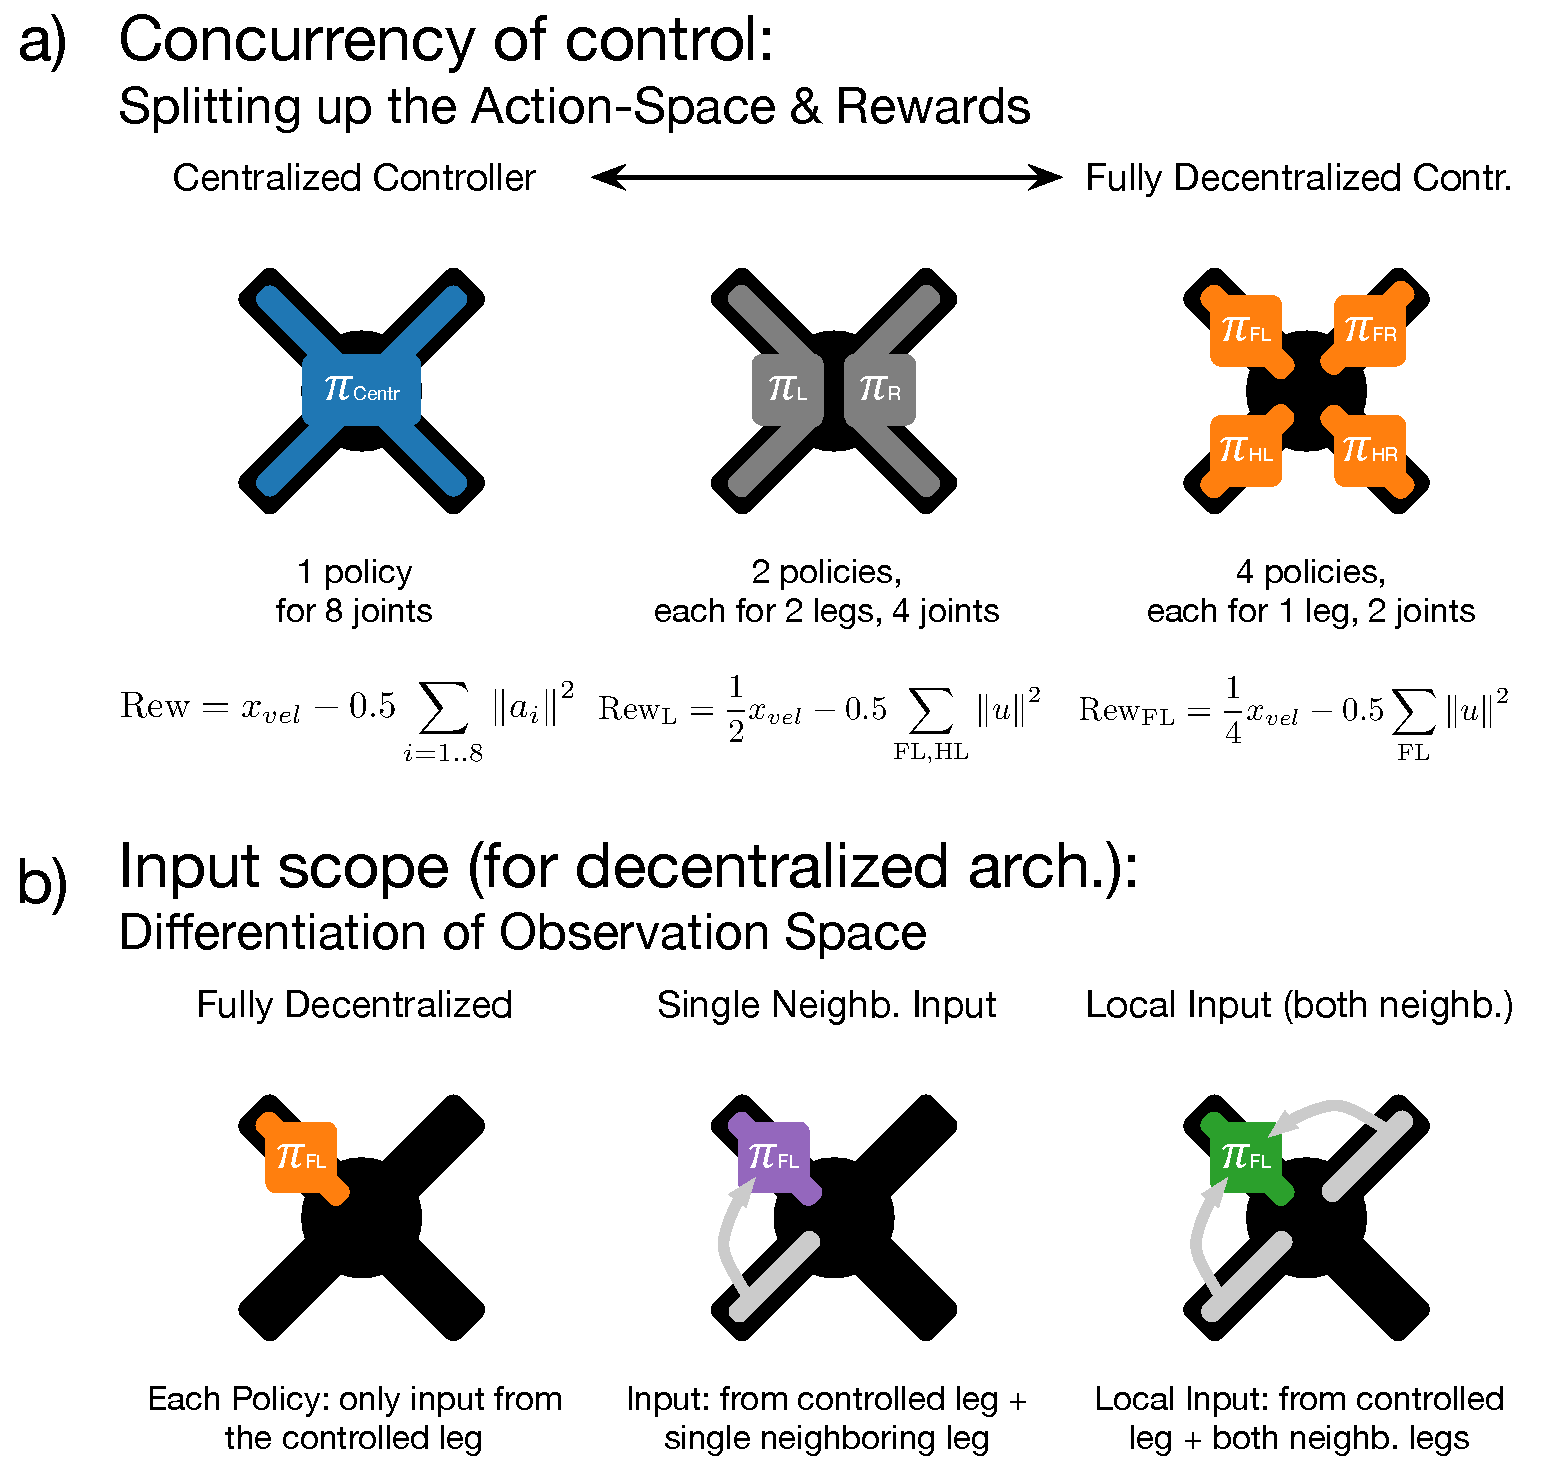
\includegraphics[width=0.5\columnwidth]{img/4-Legs Architectures.pdf}%
\caption{Example from \citep{schilling2021} -- Overview control architectures used for the four-legged simulated robot. As a first differentiation, we distinguish concurrency for which the spectrum of different architectures is shown in a). In the centralized case (left), a single controller relying on all available information learns how to control all eight joints. Training is driven by one combined reward (shown is in all cases a simplified reward, not included are the external forces). Control can be split into multiple concurrent instances, e.g. one for each side (shown in the middle) or one for each leg (shown on the right, fully decentralized case). As a consequence, reward information can be more granular, e.g., only using costs associated with the joint movements of that particular leg. For a decentralized architecture, we can further distinguish the scope of information used as input to the controller (shown in b). In the fully decentralized case, the single leg controller only uses information from that particular leg and some global information (left). This scope can be broadened to include information from another leg as well (middle, there are further variations for which additional leg is providing information, not shown) or from both neighboring legs (right, called local information). Colors correspond to colors used in result sections for different types of architectures.}
\label{fig_control_arch}
\end{figure}

\begin{figure}[tb]
\centering
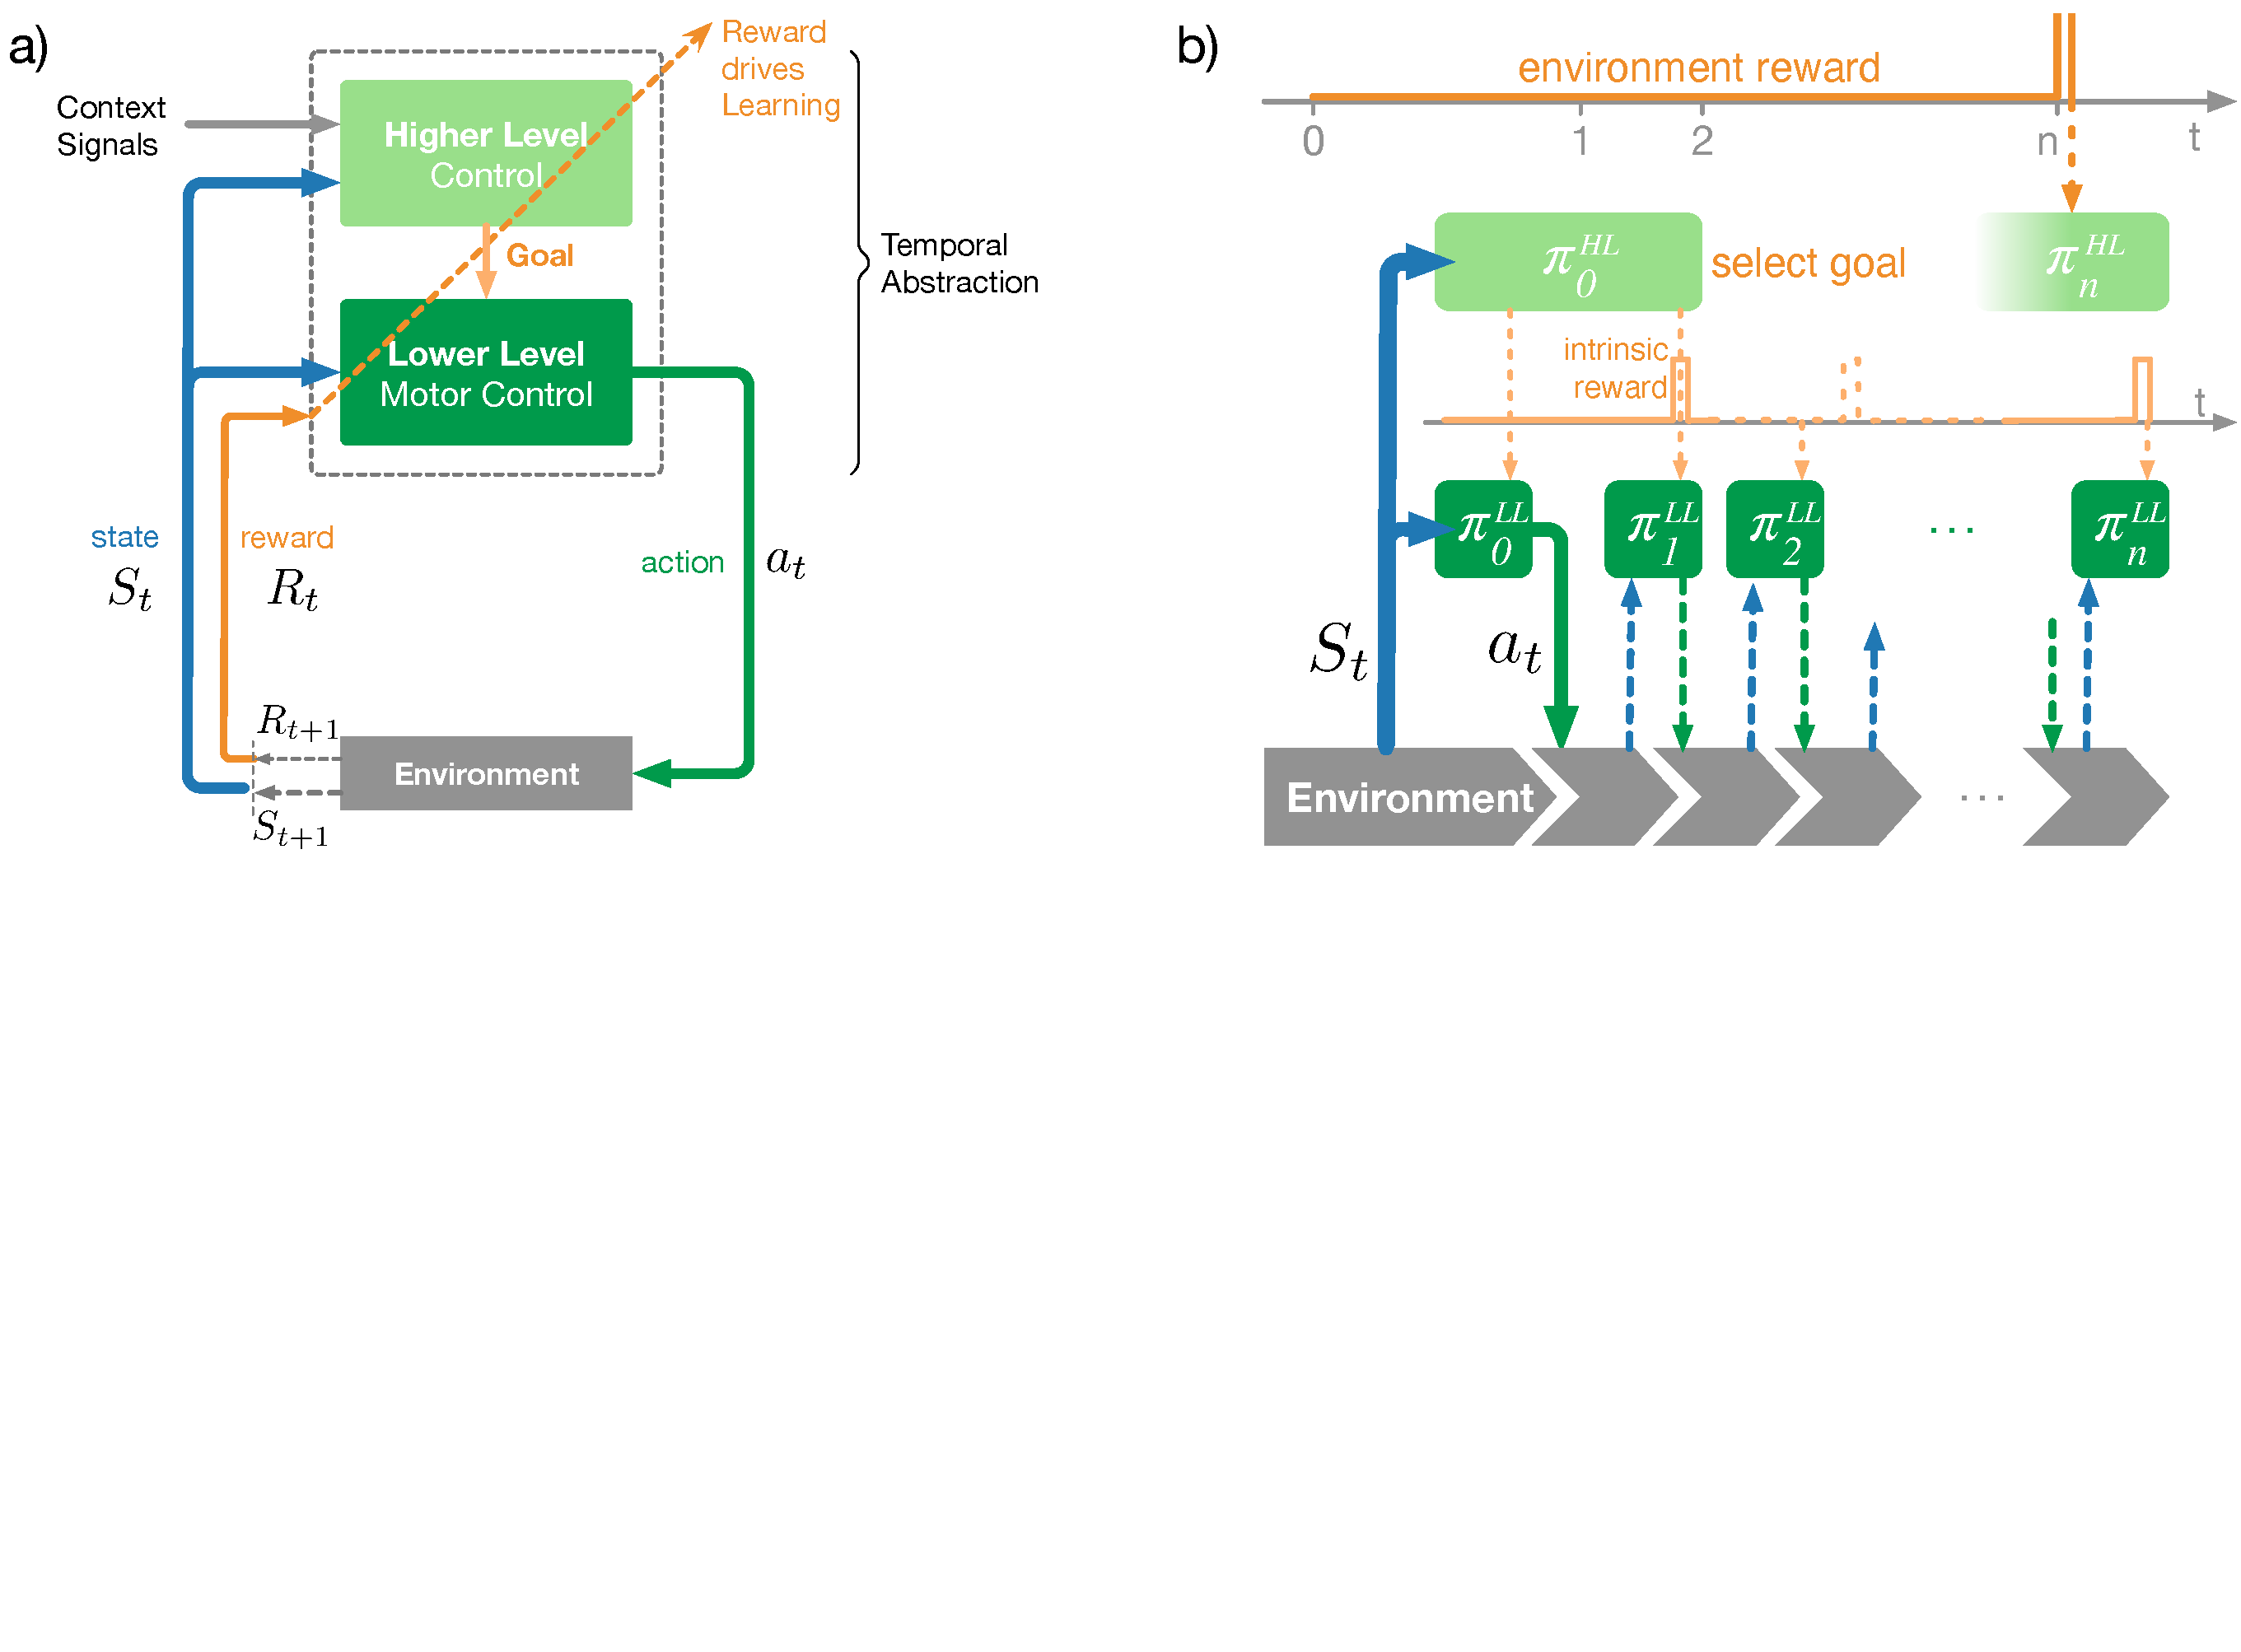
\includegraphics[width=\textwidth]{img/fig4_hrl}
\caption{Example from \citep{schilling2023} -- Conceptual view of hierarchical reinforcement learning: In panel a, the standard view of interaction with the environment in reinforcement learning is shown extended to a hierarchical perspective. For higher level control (shown in light green), this is in agreement with motor control in mammals about descending path- ways and modulation of lower level control centers. In panel b, temporal abstraction is illustrated as a process over time operating on two different levels of a hierarchy. The higher level (light green) only operates at a slow timescale being only operated every couple of time steps. The higher level aims for a sparse environmental reward. The lower level is operating on a detailed timescale each control step and providing detailed actions. It is conditioned on the higher level output which provides a form of goal context.}
\label{fig:method_example}
\end{figure}



Example images can be included to help visualize methods or results. Use the \verb+\begin{figure}+ environment to insert an image. You should ideally use vector graphics (e.g., pdf) for schematics or result plots.

\section{Mathematical Notations}
\label{s:notation}

Mathematical formulas can be set using the \verb+\begin{align}+ environment. The Bellman equation for a policy \(\pi\) is a fundamental concept in Reinforcement Learning and can be represented as follows:

\begin{align}
V^\pi(s) &= \sum_{a} \pi(a \mid s) \left( R(s,a) + \gamma \sum_{s'} P(s' \mid s,a) V^\pi(s') \right) \label{eq:bellman_policy}
\end{align}

\section{Algorithm}
\label{s:algorithm}

Algorithms are best described using pseudo-code and the \verb+algorithm+ package. Below is an example of an $\epsilon$-greedy algorithm, commonly used in Reinforcement Learning:

\begin{algorithm}
\caption{Epsilon-Greedy Algorithm}
\label{alg:epsilon_greedy}
\begin{algorithmic}
\algsetup{indent=2em}
\REQUIRE $Q(s, a)$, $\varepsilon$, $Actions$
\STATE $r \gets \text{random number}$
\IF{$r < \varepsilon$}
    \STATE $a \gets \text{random action from } Actions$
\ELSE
    \STATE $a \gets \arg\max_a Q(s, a)$
\ENDIF
\RETURN $a$
\end{algorithmic}
\end{algorithm}

\clearpage

\section{Tips for the Method Section}
\begin{itemize}
    \item Ensure that all mathematical notation is clear and consistent throughout your thesis.
    \item Describe your approach in sufficient detail to allow for replication.
    \item Use figures and tables to clarify complex concepts or results.
    \item In particular, start with an overview illustration for your architecture and consider how processes could be visualized.
    \item Provide justifications for the choices of specific methodologies or techniques.
    \item Keep the description concise but informative, focusing on why and how specific methods are chosen.
\end{itemize}

